% -----------------------------*- LaTeX *------------------------------
\documentclass[12pt]{report}
\usepackage{scribe_ee381v_modified}
\usepackage{amsmath}
\usepackage{amssymb}
\usepackage{graphicx}
%\usepackage{amsthm}
\newcommand{\set}[1]{\mathcal{#1}}
\newcommand{\rset}[1]{\mathbb{R}^{#1}}

%\newtheorem{thm}{{\bf Theorem}}
%\newtheorem{cor}{Corollary}
%\newtheorem{lem}{Lemma}
%\newtheorem{prop}{Proposition}


%\theoremstyle{remark}
%\newtheorem{rem}{Remark}

\begin{document}

% \course{CS 497}			% optional
% \coursetitle{Geometric Data Structures} % optional
% \semester{Fall 1998}			% optional
% \lecturer{Jeff Erickson}		% optional
\scribe{Jimmy Lin and Taewan Kim}		% required
\lecturenumber{16}			% required, must be a number
\lecturedate{October 21}		% required, omit year

\maketitle

% ----------------------------------------------------------------------

\section{Recap}
In the last lecture, dual of {\it Semi-Definite Programming (SDP)} problems with linear
objective function are derived as 
\begin{equation}
\begin{aligned}
    &\underset{}{\text{min}} && - \langle G, Z \rangle  \\
    &\text{ s.t.} && \langle F_i, Z \rangle = c_i,\ \forall i  \\
       & && z \succeq 0
\end{aligned}
\end{equation}
Afterwards, it is shown how to formulate following problem as linear SDP
optimization:
\begin{itemize}
    \item find a matrix with largest eigenvalue, 
    \item find sum of $r$-largest eigenvalues of a given matrix and
    \item find sum of singular values of a symmetric but not PSD matrix.
\end{itemize}
Then study of SDP is then extended to non-linear objective, which is called
{\it Log Determinant Optimization}. The general form is as follows:
\begin{equation}
\begin{aligned}
    &\underset{x}{\text{min }} && c^T x - \text{log det } G(x) \\
    &\text{ s.t.} && G(x) \succeq 0 \\
    & && F(x) \geq 0
\end{aligned}
\end{equation}
where $- \text{log det } G(x)$ is proven to be convex function. \\
Also, the following problems are formulated as Log Determinant Optimization
problem:
\begin{itemize}
    \item find the minimal-volume ellipsoid that contains all given points, 
    \item find the maximum-volume ellipsoid enclosed within a given polyhedron, 
    \item find the most likely parameters that generates a given set of samples
    \item find the variance matrix of gaussian channel with maximum capacity.
\end{itemize}
In this lecture, we will discuss {\it Proximal Gradient Algorithm}. 
Section \ref{PGA_MOTIVATION} illustrates motivations for the Proximal Gradient Algorithm. 
Section \ref{PGA_OPERATOR} will provide introduction and definition of
the Proximal Operator. 
Section \ref{PGA_ALGORITHM} gives details of the Proximal Gradient Algorithm. 
Section \ref{PGA_CONVERGENCE} is to touch convergence analysis of the Proximal
Gradient Algorithm.

\section{Motivations} \label{PGA_MOTIVATION}
As has been seen before, in order to get to $|| x - x^* || \leq \epsilon$, we
have complexity
\begin{itemize}
    \item $\mathcal{O}(\frac{1}{\epsilon})$ for gradient descent method with
        {\it smooth} objective $f(\cdot)$

    \item $\mathcal{O}(log(\frac{1}{\epsilon}))$ for gradient descent method
        with {\it strongly convex} objective $f(\cdot)$
    \item $\mathcal{O}(\frac{1}{\epsilon^2})$ for subgradient descent method
        with {\it non-smooth} objective $f(\cdot)$
\end{itemize}
\subsection{Iterative Shrinkage-Thresholding Algorithm (ISTA)}
Consider the unconstrained optimization problem with $l_1$ regularization
\begin{equation}
\begin{aligned}
    & \underset{x}{\text{ min }}
    && \frac{1}{2}\underbrace{|| y - Ax ||_2^2}_{\text{smooth/"nice"}}
    + \underbrace{  \lambda || x ||_1 }_{\text{not smooth/"nice", but "special"}}
\end{aligned}
\end{equation}
Say if $A = I$, then
\begin{equation}
\begin{aligned}
    & \underset{x}{\text{ min }} 
    && \frac{1}{2} || y - x ||_2^2 + \lambda || x ||_1 \\
    = 
    & \underset{x}{\text{ min }} 
    && \sum_i \{ \frac{1}{2} ( y_i - x_i )^2  + \lambda | x_i |_1 \} \\
\end{aligned}
\end{equation}
Obviously, such tranformation is justifiable since the original problem is
separable. \\
Now we derive closed-form solution for each "separated" problem: 
\begin{align}
    x_i-y_i + \lambda & && \text{ if } x_i > 0 \\
    x_i-y_i - \lambda & && \text{ if } x_i < 0 \\
    -y_i + r \lambda &, r \in (-1,1) && \text{ if } x_i = 0 
\end{align}
Suppose $y_i > 0$, then it obvious that $x_i \geq 0 $. 
\begin{itemize}
    \item if $x_i > 0$, then $\exists x_i = y_i - \lambda$.
    \item if $x_i = 0$, then 
\end{itemize}
Similarly, if $y_i < 0$, then exists $x_i = y_i + \lambda$ if $x_i < 0$.
% TODO: add figure here

\subsection{Motivation 2}
Consider another optimization problem
\begin{equation}
\begin{aligned}
    &  \underset{x}{\text{ min }}
    && \underbrace{g(x)}_{\text{"nice"}} \\
    &  \text{ s.t. } 
    && x \in Q
\end{aligned}
\end{equation}
where $Q$ is a convex set and is easy to project onto, e.g. $Q: \{ x| ||x||_{\infty} \leq 1 \}$. \\
The above optimization problem equates to 
\begin{equation}
\begin{aligned}
    &  \underset{x}{\text{ min }}
    && g(x) + I_Q(x) 
\end{aligned}
\end{equation}
where 
\begin{equation}
    I_Q (x) = 
   \begin{cases}
   0 &\mbox{if } x \in Q  \\
   \infty &\mbox{if } x \not \in Q
   \end{cases}
  \end{equation}
Hence, we have 
\begin{equation}
    [P_Q(y)]_i =
   \begin{cases}
   y_i &\mbox{if } |y_i| \leq 1  \\
   sign(y_i) &\mbox{otherwise} 
   \end{cases}
  \end{equation}
  
\section{Proximal Operator} \label{PGA_OPERATOR}
Proximal gradient is an algorithm for unconstrained problems with a cost function which can be expressed sum of two functions.
\begin{equation}
\textrm{minimize}~f(x)=g(x)+h(x)
\end{equation}
\vspace{-2.5em}
\begin{align*}
g(x)&: \textit{'nice'}, \text{ (ex) convex, L-lipschitz gradient}\\
h(x)&: \textit{'special'}, \text{ (ex) convex, not smooth, \textbf{prox} is easy to calculate}
\end{align*}

In the above equation, we used the term 'nice' and 'special' to express the characteristic of each function $g$ and $h$. Specific conditions on $g$ and $h$ will be more clear in the theorem which will be provided later. And the following is a definition of prox function (proximal operator) which clarifies the meaning of \textbf{prox} in the condition of $h$.

\begin{definition}\textbf{\em{(Prox function/ Proximal operator)}}\\
The prox function (or proximal operator) of a function $h(\cdot)$ is defined as:
\begin{equation}
\textbf{\em{prox}}_{th}(v) = \arg\min_{x} \left( h(x)+\frac{1}{2t}\|x-v\|_2^2 \right)
\end{equation}
\end{definition}

One natural example of proximal operator is projection on set $Q$. Suppose you perform a gradient descent and require a solution to be in a certain set $Q$. So, in each step, $x_{+}$ should satisfy the condition $x_{+}\in Q$, and this can be done by using projection $P_Q$ as in Figure \ref{16fig:projection}.
\begin{figure}[t]
    \centering
    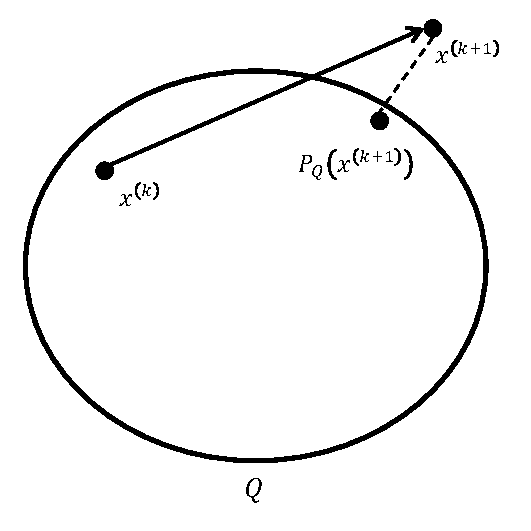
\includegraphics[scale=0.8]{L16_fig_projection}\\
    \caption{Projection on $Q$ for gradient step}\label{16fig:projection}
\end{figure}
\begin{equation}
x^{(k+1)} = P_Q \left( x^{(k)}-t \nabla g(x^{(k)})\right)
\end{equation}
And this projection operator is a specific version of proximal operator by using $h(x)=I_Q (x)$ where $I_Q(\cdot )$ is a indicator function of $Q$.
\begin{align*}
\textbf{prox}_h (x) &= \arg\min_u \left( h(u) + \frac{1}{2}\|u-x\|_2^2 \right)\\
&= \arg\min_u \left( I_Q (u) + \frac{1}{2}\|u-x\|_2^2 \right)\\
&= \arg\min_{u \in Q} \left( \frac{1}{2}\|u-x\|_2^2 \right)\\
&= P_Q (x)
\end{align*}
where indicator function $I_Q$ is defined as, 
\begin{equation*}
I_Q (x) =  \begin{cases}
	0 & \text{if}~x \in Q \\
	\infty & \text{if}~x \notin Q
	\end{cases}  
\end{equation*}
Third equality comes from the fact that $u\notin Q$ gives infeasible solution $x$ for minimizing the function. And the last equality is the general definition of projection based on the Euclidean distance.

\section{Proximal Gradient Algorithm} \label{PGA_ALGORITHM}
Now we can introduce a proximal gradient algorithm which uses two black boxes, one outputs $\nabla g(x)$ and the other outputs $\textbf{prox}_{th}(v)$ (Figure \ref{16fig:twoblackboxes}), for the task of minimizing $f(x) = g(x) + h(x)$.
\begin{figure}[ht]
    \centering
    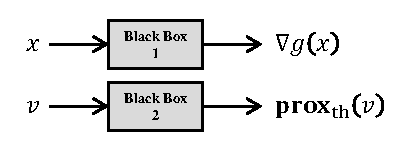
\includegraphics[scale=1]{L16_fig_twoblackboxes}\\
    \caption{Using two black boxes for proximal gradient}\label{16fig:twoblackboxes}
\end{figure}

\vspace{1em}
\noindent\textbf{- Proximal Gradient Algorithm}\\
Proximal gradient algorithm is defined as the following update rule.
\begin{equation}
x_+ \leftarrow \textbf{prox}_{th} \left(x - t\nabla g(x) \right)
\end{equation}

By using the definition of proximal operator, update of proximal gradient can be expressed as follows:
\begin{align}
x_+ &\leftarrow \textbf{prox}_{th} \left(x - t\nabla g(x) \right)\nonumber\\
&= \arg\min_u \left( h(u)+\frac{1}{2t}\|u-x+t\nabla g(x)\|_2^2 \right)\nonumber\\
&= \arg\min_u \left( h(u)+\langle \nabla g(x), u-x \rangle + \frac{1}{2t}\|u-x\|_2^2 +\frac{t}{2}\| \nabla g(x) \|_2^2 \right)\nonumber\\
&= \arg\min_u \left( h(u)+\langle \nabla g(x), u-x \rangle + \frac{1}{2t}\|u-x\|_2^2 + g(x) \right)
\end{align}\label{16eq:prox_quadratic}
Last equality comes from the fact that $\| \nabla g(x) \|_2^2$ and $g(x)$ do not depend on $u$. In equation (\ref{16eq:prox_quadratic}), an important fact to point out is that rear part has a form of quadratic approximation of $g(u)$ around $x$.
\begin{equation}
g(x) + \langle \nabla g(x), u-x \rangle + \frac{1}{2t}\|u-x\|_2^2 
\end{equation} 

\section{Convergence Analysis} \label{PGA_CONVERGENCE}
The convergence of proximal gradient algorithm requires $O(1/\epsilon)$ of iteration. Following theorem specifies the condition and time complexity.

\begin{theorem}\label{16thm:convergence}
If $g$ is convex and $g$ has L-lipschitz gradient, i.e. $\| \nabla g(x) - \nabla g(y)\|_2 \leq L\|x-y\|_2$, using fixed size $t < 1/L$ on proximal gradient algorithm gives $O(1/\epsilon)$ of convergence to the optimal point $x^*$, where $x^* = \arg\min_x \left( g(x) + h(x)\right)$.
\end{theorem}

Before providing a proof of the theorem, let's define a function $G_t (x)$ which satisfies the following condition. Role of the $G_t(x)$ function is to remove the proximal operator on the whole equation and make it similar to the general update as before.
\begin{align*}
x_+ &\leftarrow x-t G_t (x)=\textbf{prox}_{th}(x-t\nabla g(x))\\
\Leftrightarrow G_t (x) &\triangleq \frac{1}{t}\left( x - \textbf{prox}_{th}(x-t\nabla g(x)) \right)
\end{align*}

\noindent\textbf{Claim 1.} $G_t (x)- \nabla g(x) \in \partial h(x-tG_t (x))$

\begin{lemma}
\label{16lemma:quadratic} 
For any point $z$, $f(x_+)\leq f(z)+ \langle G_t (x),x-z \rangle -\frac{t}{2}\|G_t (x)\|_2^2 $
\end{lemma}
Proof of Claim 1 and Lemma \ref{16lemma:quadratic} is provided after the proof of Theorem \ref{16thm:convergence}.

\begin{proof}[Theorem \ref{16thm:convergence}]
Putting $z=x$ in the Lemma \ref{16lemma:quadratic} gives,
\begin{equation*}
f(x_+) \leq f(x)-\frac{t}{2}\|G_t (x)\|_2^2
\end{equation*}
So, this gives the decreasing property $f(x_+) \leq f(x)$ since step size satisfies $t \geq 0$. 
And putting $z=x^*$ gives,
\begin{align*}
f(x_+) &\leq f^*-\frac{t}{2}\|G_t (x)\|_2^2+\langle G_t (x),x-x^* \rangle\\
\Leftrightarrow f(x_+)-f^* &\leq \frac{1}{2t}\left[ \|x-x^* \|_2^2 - \|x-x^*-tG_t(x)\|_2^2 \right]\\
&=\frac{1}{2t}\left[ \|x-x^* \|_2^2 - \|x_+ -x^*\|_2^2 \right]
\end{align*}
Adding up over $T$ iterations gives
\begin{align*}
\sum_{k=1}^{T}\left(f(x^{(k)})-f^* \right) &\leq \frac{1}{2t} \left[\|x^{(0)}-x^*\|_2^2 - \|x^{(T)}-x^*\|_2^2\right] \\
&\leq \frac{1}{2t}\|x^{(0)}-x^*\|_2^2
\end{align*}

From the fact that $f(x_+) \leq f(x)$ as shown above, $f(x^{(k)})-f^* \geq f(x^{(T)})-f^*$ for $k=1,\cdots T$. And this gives,
\begin{equation*}
f(x^{(T)})-f^* \leq \frac{1}{2tT} \|x^{(0)}-x^*\|_2^2
\end{equation*}
which concludes the proof of $O(1/\epsilon)$ convergence, i.e. it requires $k= O(1/\epsilon)$ of iteration number to have $f(x^{(k)})-f^* \leq \epsilon$.

\end{proof}

\begin{proof}[Lemma \ref{16lemma:quadratic}]
From the L-lipschitz continuous of gradient on $g$,
\begin{equation*}
g(y) \leq g(x) + \langle \nabla g(x),y-x \rangle +\frac{L}{2}\|y-x\|_2^2
\end{equation*}
So, for $y=x_+=x-tG_t(x)$
\begin{equation}\label{16eq:lemma_proof1}
g(x_+) \leq g(x)- \langle \nabla g(x), tG_t(x) \rangle +\frac{L}{2}t^2 \|G_t(x)\|_2^2
\end{equation}
And recall the condition of subgradient. If $a \in \partial h(x_+)$ then,
\begin{equation*}
h(z) \geq h(x_+)+\langle a,z-x_+ \rangle
\end{equation*}
From the Claim 1, $G_t(x)-\nabla g(x) \in \partial h(x-tG_t(x))$. By setting $a=G_t(x)-\nabla g(x)$ gives,
\begin{align}
h(z) &\geq h(x_+) + \langle G_t(x) -\nabla g(x),z-x_+ \rangle \nonumber\\
\Leftrightarrow ~h(x_+)&\leq h(z)-\langle G_t(x) -\nabla g(x),z-x_+ \rangle
\label{16eq:lemma_proof2}
\end{align}
Now using $f(x_+)=g(x_+)+h(x_+)$, and adding (\ref{16eq:lemma_proof1}) and (\ref{16eq:lemma_proof2}):
\begin{align*}
f(x_+) \leq ~&g(x)- \langle \nabla g(x), tG_t(x) \rangle +\frac{L}{2}t^2 \|G_t(x)\|_2^2\\
&+h(z)-\langle G_t(x) -\nabla g(x),z-x_+ \rangle\\
\leq ~&g(z) -\langle \nabla g(x),z-x \rangle - \langle \nabla g(x), tG_t(x) \rangle +\frac{L}{2}t^2 \|G_t(x)\|_2^2\\
&+h(z)-\langle G_t(x) -\nabla g(x),z-x_+ \rangle \\
&\hspace{3em}(\because g(x) \leq g(z)-\langle \nabla g(x),z-x \rangle \text{ from convexity of } g)\\
= ~&f(z)-\langle \nabla g(x),z-x+tG_t(x)-(z-x_+) \rangle\\
&+\frac{L}{2}t^2 \|G_t(x)\|_2^2 - \langle G_t(x),z-x_+ \rangle\\
= ~&f(z)+\frac{L}{2}t^2 \|G_t(x)\|_2^2 - \langle G_t(x),z-x+tG_t(x) \rangle\\
\leq ~&f(z)+\langle G_t (x),x-z \rangle+\frac{t}{2}\|G_t(x)\|_2^2-t \|G_t(x)\|_2^2 \hspace{2em}(\because t<1/L)\\
= ~&f(z)+\langle G_t (x),x-z \rangle-\frac{t}{2}\|G_t(x)\|_2^2
\end{align*}
This concludes the proof of Lemma \ref{16lemma:quadratic}.
\end{proof}

Remaining part is the proof of Claim 1, i.e. $G_t (x)- \nabla g(x) \in \partial h(x-tG_t (x))$.

\begin{proof}[Claim 1]
To show that $G_t(x)-\nabla g(x)$ is a subgradient of $h(x-tG_t(x))=h(x_+)$, let's show that the following property of proximal operator is true.
\begin{equation}\label{16eq:claim1_sub}
u=\textbf{prox}_{th}(x) \Leftrightarrow \frac{1}{t}(x-u) \in \partial h(u)
\end{equation}
Proof of the property (\ref{16eq:claim1_sub}) is based on the definition of proximal operator, which means that $\textbf{prox}_{th}(x)$ is a minimizer.
\begin{gather*}
\frac{1}{t}(x-u) \in \partial h(u)\\
\Leftrightarrow h(u)+\langle \frac{1}{t}(x-u),y-u \rangle \leq h(y), ~~\forall y\\
\Leftrightarrow h(u)+\langle \frac{1}{t}(x-u), y-u \rangle -\frac{1}{2t}\|y-u\|_2^2 \leq h(y)-\frac{1}{2t}\|y-u\|_2^2 \leq h(y), ~~\forall y\\
\Leftrightarrow h(u) + \langle \frac{1}{t}(x-u)+\frac{1}{2t}(u-y),y-u \rangle \leq h(y), ~~\forall y\\
\Leftrightarrow h(u)+\frac{1}{2t}\langle 2(x-u) +(u-y), (x-u)-(x-y) \rangle \leq h(y),~~\forall y\\
\Leftrightarrow h(u)+\frac{1}{2t}\langle (x-u) +(x-y), (x-u)-(x-y) \rangle \leq h(y),~~\forall y\\
\Leftrightarrow h(u)+\frac{1}{2t}\left(\|u-x\|_2^2-\|y-x\|_2^2 \right) \leq h(y),~~\forall y\\
\Leftrightarrow h(u)+\frac{1}{2t}\|u-x\|_2^2 \leq h(y)+\frac{1}{2t}\|y-x\|_2^2,~~\forall y\\
\Leftrightarrow u = \arg\min_{z} \left( h(z)+\frac{1}{2t}\|z-x\|_2^2 \right)\\
\Leftrightarrow u=\textbf{prox}_{th}(x)
\end{gather*}

Now put $u=x_+ = \textbf{prox}_{th}(x-\nabla g(x))$ in equation (\ref{16eq:claim1_sub}).
\begin{align*}
\Rightarrow ~&\frac{1}{t}(x-\nabla g(x) - x_+) \in \partial h(x_+)\\
\Rightarrow ~&\frac{1}{t}(x-\nabla g(x) - x+tG_t(x)) \in \partial h(x_+)\\
\Rightarrow ~&G_t(x) -\nabla g(x) \in \partial h(x_+)
\end{align*}

\end{proof}


\end{document}

